%% 4-PSK Modulation Constellation
\subfloat[QPSK]{
\begin{tikzpicture}[scale=2.2]

    \def\cos45{0.7071}
    \colorlet{anglecolor}{black}

    \draw[dashed] (0,0) circle (1cm);

    \draw[->] (-1.3,0) -- (1.3,0) node[below] {$I$};
    \draw[->] (0,-1.3) -- (0,1.3) node[right] {$Q$};

     \draw[draw=anglecolor] (0,0) -- (3mm,0pt) arc(0:45:3mm);
     \draw (15:5mm) node[anglecolor, font=\footnotesize] {$\pi/4$};
     \filldraw [black] (\cos45, \cos45) circle(1pt)
                     (-\cos45, -\cos45) circle(1pt)
                     (\cos45, -\cos45)  circle(1pt)
                     (-\cos45, \cos45)  circle(1pt);

     \draw[->] (0,0) -- (\cos45, \cos45);
     \draw (45:1cm) node[right=2pt, font=\footnotesize] {$00$};
     \draw (-45:1cm) node[right=2pt, font=\footnotesize] {$01$};
     \draw (135:1cm) node[left=2pt, font=\footnotesize] {$10$};
     \draw (225:1cm) node[left=2pt, font=\footnotesize] {$11$};
\end{tikzpicture}
} \qquad
\subfloat[8-PSK]{
%% 8-PSK Modulation Constellation
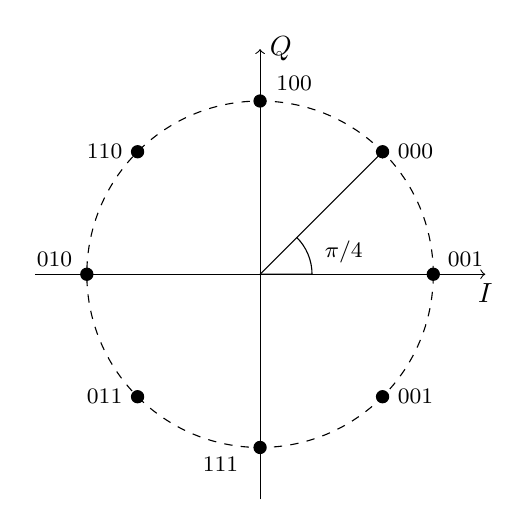
\begin{tikzpicture}[scale=2.2]

    \def\cos45{0.7071}
    \colorlet{anglecolor}{black}

    \draw[dashed] (0,0) circle (1cm);

    \draw[->] (-1.3,0) -- (1.3,0) node[below] {$I$};
    \draw[->] (0,-1.3) -- (0,1.3) node[right] {$Q$};

     \draw[draw=anglecolor] (0,0) -- (3mm,0pt) arc(0:45:3mm);
     \draw (15:5mm) node[anglecolor, font=\footnotesize] {$\pi/4$};
     \filldraw [black] (\cos45, \cos45) circle(1pt)
                     (-\cos45, -\cos45) circle(1pt)
                     (\cos45, -\cos45)  circle(1pt)
                     (-\cos45, \cos45)  circle(1pt)
                     (-1,0)             circle(1pt)
                     (1,0)             circle(1pt)
                     (0,1)             circle(1pt)
                     (0,-1)             circle(1pt);

     \draw[->] (0,0) -- (\cos45, \cos45);
     \draw (45:1cm) node[right=2pt, font=\footnotesize] {$000$};
     \draw (88:1.1cm) node[right, font=\footnotesize]    {$100$};
     \draw (5:1cm) node[right=2pt, font=\footnotesize]       {$001$};
     \draw (175:1cm) node[left=2pt, font=\footnotesize]  {$010$};
     \draw (-45:1cm) node[right=2pt, font=\footnotesize] {$001$};
     \draw (135:1cm) node[left=2pt, font=\footnotesize] {$110$};
     \draw (225:1cm) node[left=2pt, font=\footnotesize] {$011$};
     \draw (268:1.1cm) node[left=2pt, font=\footnotesize] {$111$};
\end{tikzpicture}
}

